%!TEX root = main.tex

% https://tex.stackexchange.com/questions/24066/start-new-chapter-on-same-page/24068#24068
{
\let\clearpage\relax

\chapter{Models}
}

\section{Hierarchical models}

The player and enemy characters are represented by complex models that include a hierarchy of bones to drive the animation of different parts of the mesh.

\subsection{Makoto, the player character}

The model for the player character is named \textit{Makoto} and has the form of a stylized human holding a sword. The model and its bones are shown in \autoref*{fig:makoto-bones}.\footnote{The bones have been enlarged in order to make it possible to see them in the first place. In the real model, all bones are point-like and pointing up.}

\begin{figure}[H]
    \centering
    \includesvg[width=\textwidth]{images/ch3/Grafo-Makoto.svg}
    \caption{Hierarchy tree of Makoto's bones}
    \label{fig:makoto-graph}
\end{figure}

\begin{wrapfigure}[23]{r}{0.4\textwidth}
    \centering
    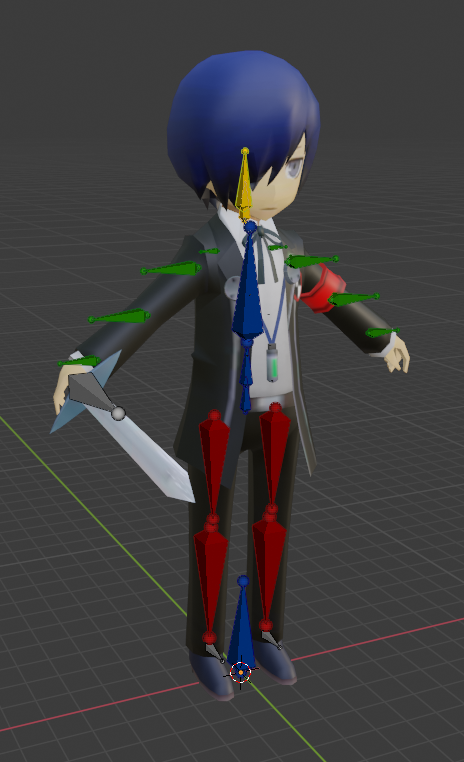
\includegraphics[width=0.4\textwidth]{images/ch3/Makoto-Bones-v2.png}
    \caption{Makoto's model with his bones shown. The bones have been colored by group (root and spine, legs, arms, head)}
    \label{fig:makoto-bones}
\end{wrapfigure}

Makoto's model is made of one mesh which is fully UV-mapped to one color texture. We also generated a roughness map from that texture in order to make the sword in his hand and the earphones around his shoulder shinier and more metallic-looking, although this effect is hard to see.

Because half of Makoto's face is covered by his hair, we used this model flipped along the X axis in order to make his better profile visible in the default view of the battle scene, where the player is placed on the left side of the screen and facing right.

The animation of the mesh is driven by the hierarchy of bones described in \autoref*{fig:makoto-graph}. They are directly mapped to TransformNode and Bone objects in the Babylon environment. Specifically, this is a list of the relevant bones for animating:

\begin{itemize}
    \item \textbf{rot} and \textbf{Bip01} are the top nodes. The former is located at the base of the model, the latter approximately at his waist.
    \item \textbf{Bip01_Spine} and \textbf{Bip01_Spine1} control the torso and chest.
    \item \textbf{Bip01_L_Thigh}, \textbf{Bip01_L_Calf} and \\ \textbf{Bip01_L_Foot} control the respective parts of the left leg. Similarly for the right counterparts.
\end{itemize}

\begin{itemize}
    \item \textbf{Bip01_L_Clavicle}, \textbf{Bip01_L_UpperArm}, \textbf{Bip01_L_Forearm} and \\ \textbf{Bip01_L_Hand} control the corresponding parts of the left arm. Similarly for the right counterparts.
    \item \textbf{weapon} controls the sword.
    \item \textbf{Bip01_Neck} and \textbf{Bip01_Head} control the head.
\end{itemize}

The model came with a larger number of nodes, but we felt that the others were either too close to the ones we had already chosen or outright irrelevant for animation.


\subsection{Samurai, the common enemy}

The common, weaker enemy that is encountered multiple times throughout the dungeon is represented by a model of a masked, armored Samurai wielding a long katana. The model and its bones can be seen in \autoref*{fig:samurai-bones}.\footnote{Like for Makoto, the bones have been enlarged for illustration purposes}

The Samurai's model is made of a mesh mapped to two color textures, roughly one for the main body and one for accessories such as the sword and the ornament on top of the helmet. Therefore, it translates to two meshes in Babylon. We also generated a roughness map to represent the metallic parts of the model, i.e. the sword and the golden ornament on top of the helmet, by making them shinier; and we created an emissive texture to make those same elements glow in the dark when the Samurai uses its special attack.

The bone hierarchy of the Samurai features a humanoid base identical to Makoto's (apart from the name of a few bones), and a number of additional bones:

\begin{itemize}
    \item The "\textbf{mant}" bones are organized in three 2-bone chains and animate a cape behind the Samurai's back
    \item The four "\textbf{maekake}" bones control that many pieces of armor around the enemy's waist, which would otherwise penetrate with the legs as they move
\end{itemize}

The bones of this model are directly mapped to Babylon TransformNodes and Bones upon importing. The hierarchy of the Samurai is detailed in \autoref*{fig:samurai-graph}.

\begin{figure}[H]
    \centering
    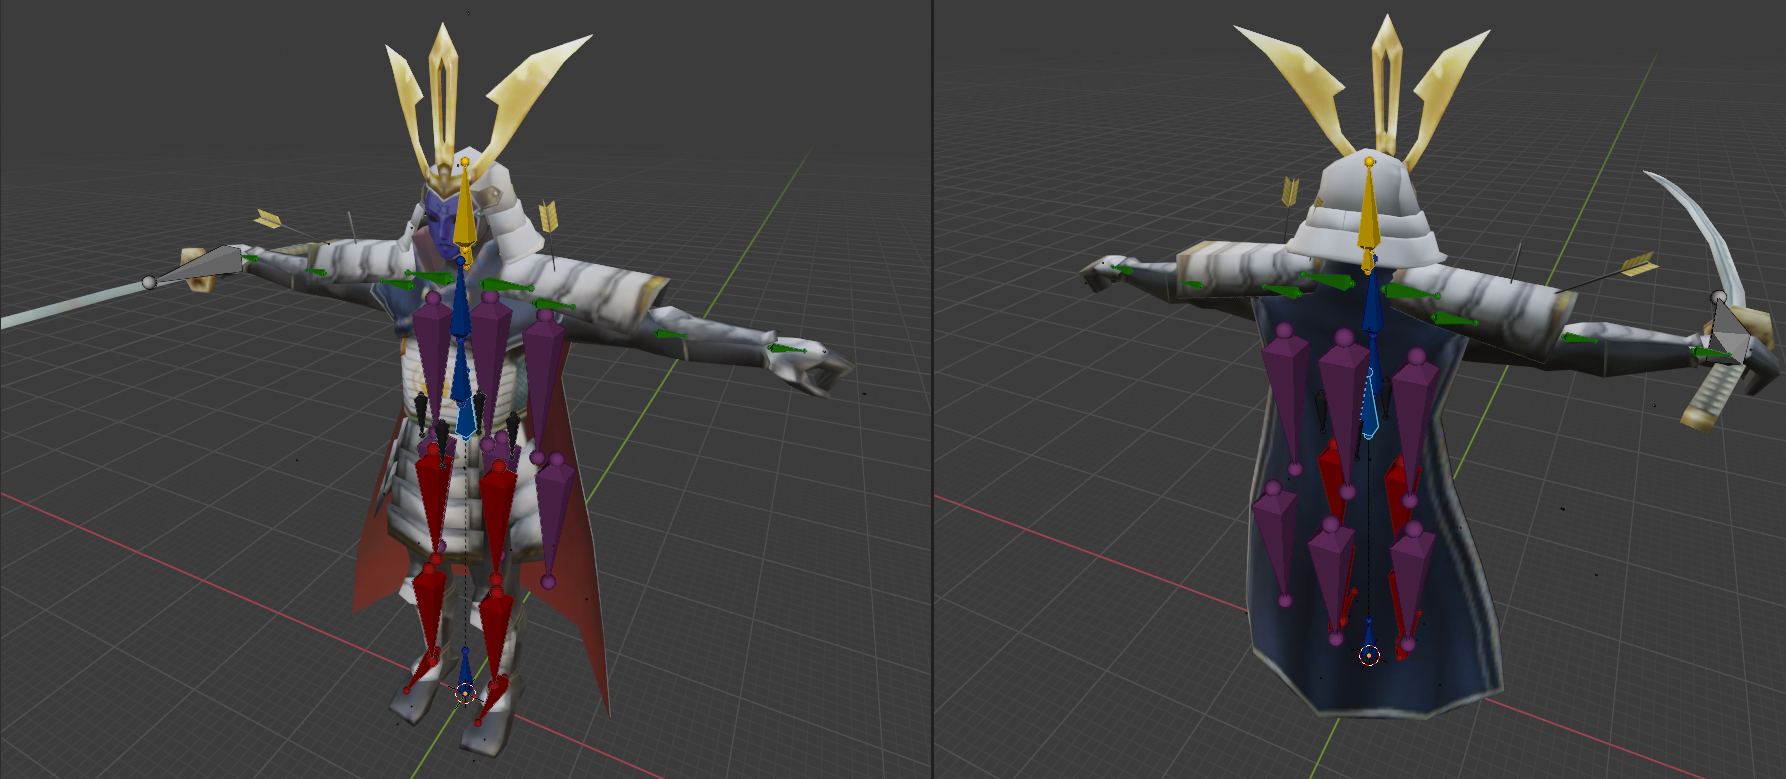
\includegraphics[width=1\textwidth]{images/ch3/Samurai-Bones.png}
    \caption{The Samurai's model with its bones shown. Frontal and back view. The bones have been colored by group (root and spine, legs, arms, head, cape, waist armor)}
    \label{fig:samurai-bones}
\end{figure}

\begin{figure}[H]
    \centering
    \includesvg[width=\textwidth]{images/ch3/Grafo-Samurai.svg}
    \caption{Hierarchy tree of the Samurai's bones. The blue scroll-like shapes indicate parts of the hierarchy that are identical to Makoto's corresponding parts as shown in \autoref{fig:makoto-graph}, so they were omitted to simplify this graph.}
    \label{fig:samurai-graph}
\end{figure}


\subsection{The Boss enemy}

The final, stronger enemy found at the end of the dungeon, commonly referred to as the "boss", is represented by a model of a masked, slightly abstract demon with a large cape. This enemy is referred to as "Evil Lord of Shadows" in the game, while in the code it is called "Phantom Master", which is the original name of the model and the working name we used before settling on the final one. The model and its bones can be seen in \autoref*{fig:phantom-bones}.\footnote{Yet again, the bones have been enlarged for illustration purposes}

The model is made of a mesh mapped to four color textures: the mask, the body, the cape, and the flame in the lantern. This results in the Babylon glTF importer creating four meshes to represent this model.

The bone hierarchy of the model from its waist up is similar to the other humanoid models, but:

\begin{itemize}
    \item The equivalent of its legs have a more simplified hierarchy, meaning they cannot be controlled independently, and they lack a "knee" joint. Therefore, we treated the legs like a fixed part.
    \item The cape has its own root node, which is child of the upper spine node, and six bone chains that control the different parts of the cape. The chains are 2 or 3 bones long each, but we always focused on the first two nodes of each since the later ones did not seem relevant for our animations.
\end{itemize}

The bones of this model are directly mapped to Babylon TransformNodes and Bones upon importing. The hierarchy of the boss is detailed in \autoref*{fig:phantom-graph}.

\begin{figure}[H]
    \centering
    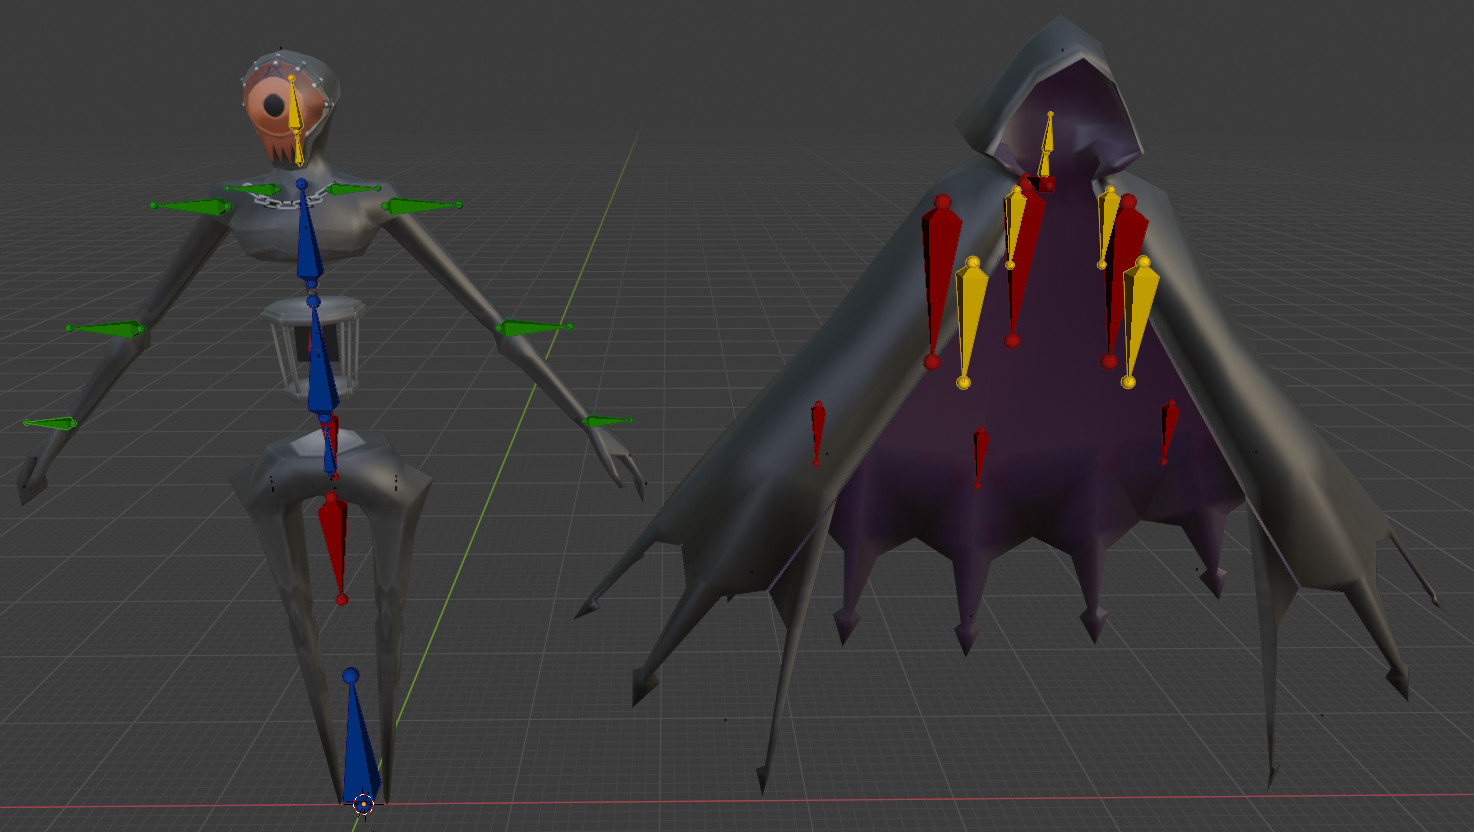
\includegraphics[width=1\textwidth]{images/ch3/Phantom-Bones.png}
    \caption{Boss model with its bones shown. Body and cape have been separated. The bones have been colored by group (root and spine, legs, arms, head, cape front, cape back)}
    \label{fig:phantom-bones}
\end{figure}

\begin{figure}[H]
    \centering
    \includesvg[width=\textwidth]{images/ch3/Grafo-Phantom.svg}
    \caption{Hierarchy tree of the boss's bones. The blue scroll-like shapes indicate parts of the hierarchy that are identical to Makoto's corresponding parts as shown in \autoref{fig:makoto-graph}, so they were omitted to simplify this graph.}
    \label{fig:phantom-graph}
\end{figure}

\newpage

\section{Other models}

Most other objects in the dungeon are represented by other, simpler glTF models.

\subsection{Floor and Wall}

The basic building blocks of the dungeon are these two modular tiles that, when replicated through instancing, make up the entirety of the dungeon's floor and walls. Both tiles are square and have an irregular surface, as if it was made of bricks.

Each tile was assigned a different set of color, diffuse, and roughness textures to give the appearance of two different construction materials.

\subsection{Arch}

An archway found in the dungeon, usually to contain doors or bars. It was assigned the same set of texture as the wall, for continuity.

\subsection{Door}

A simple wooden door with metallic reinforcements. It is worth noting that its pivot is on one of its lateral sides, thus allowing it to open simply by changing its rotation.

It was assigned a diffuse texture that is just a palette of uniform colors, which let us set a single material for the whole mesh and thus avoid that Babylon split the door into multiple meshes, since it allows only one material per mesh. The door was also given a normal and a roughness texture to give the appearance of wood and metal.

\subsection{Bars}

A simple set of metal bars in a grid. We decided that they needed no textures.

\subsection{Lock}

A padlock that goes on a set of bars to show they are locked.

It was assigned a palette of uniform colors as a texture to give it two tones of color. Those colors are merely shades of gray in order to allow the Babylon code to assign a different base color to each clone of the lock mesh.

\subsection{Keys}

The items that open the locks. We included two variant meshes for the keys: one for the common keys and a second, more elaborate one for the key to the boss room.

\subsection{Spike trap}

Composed of two meshes: a base tile and the sharp, pointy spikes that come out of it when the player gets too close. Although establishing a hierarchy between the two meshes may sound intuitive, we decided not to make the spikes a child of the base in order to facilitate the instantiation process in Babylon, and also because the base is static.

Both meshes were assigned color, normal and roughness textures to give the appearance of dirty metal.

\subsection{Props}

A number of purely decorative items, including:

\begin{itemize}
    \item \textbf{Table and chairs}, which were given color, normal, and roughness textures to give the appearance of wood with some metallic parts. The wood texture was made darker and given some shade of red on purpose in order to contrast against the wall.
    \item \textbf{Wall banners}, which were divided into two meshes: a base, and the banner itself. The former was given a palette of uniform colors, the latter was given nothing in order to let the JS code color each clone separately.
    \item \textbf{Open and empty chest}, which was given a palette of uniform colors and a normal texture, like the door.
    \item \textbf{Wall mount for swords}, which was given a palette of uniform colors and a normal and roughness texture to simulate both the wood of the stand and the metallic shininess of the swords.
    \item \textbf{Cobweb}, a simple mesh to decorate some corners.
    \item \textbf{Skull}, a simple mesh to decorate various point of the dungeon and the battle arena.
    \item \textbf{Pedestal}, used only in the ending to hold the Cube of Babylon. It was given color, normal and roughness textures for a marble-like appearance.
    \item \textbf{The Cube of Babylon}, used only in the ending. It was given no textures: its two colors are given by two different materials. This choice was made for simplicity and because the ending had less performance concerns.
\end{itemize}